
\documentclass[12pt]{amsart}
\usepackage{geometry} % see geometry.pdf on how to lay out the page. There's lots.
\geometry{a4paper} % or letter or a5paper or ... etc
% \geometry{landscape} % rotated page geometry
\usepackage[utf8]{inputenc}

\usepackage{booktabs}

\usepackage[pdftex]{graphicx}

% See the ``Article customise'' template for come common customisations

\title{Blatt 12}
\author{Dora Szücs und Sarah Köhler}
%\date{} % delete this line to display the current date

%%% BEGIN DOCUMENT
\begin{document}

\maketitle
%\tableofcontents

\section*{Aufgabe 4.2 Arbeitsplanung}

Der Graph in Abb. 1 illustriert das Flussproblem, dass sich aus der Aufgabenstellung ergibt: Die Arbeiter bilden einen Teil der Knoten, die Dienstleistungen den anderen Teil der Knoten eines bipartiten Graphen. Zudem sind eine Quelle und eine Senke nötig.
Alle Arbeiter haben arbeiten maximal 8 Stunden am Tag, deswegen ist dies die Kapazität die von der Quelle (S) zu den einzelnen Arbeitern gegeben ist. Die Nachfrage dagegen bestimmt die Kapazitäten der ausgehenden Kanten von den Dienstleistungenn zur Senke (T). 
Die Kanten von den Arbeitern zu den einzelnen Dienstleistungen zeigen an, welche Arbeiter welche dieser Diensteilungen ausführen können. Die dort angegebenen Kapazitäten entsprechen der maximalen Zeit, die ein Arbeiter am Tag diese Dienstleistung ausführen kann, was genau der maximalen Arbeitszeit von 8 Stunden entspricht.

\begin{figure}[ht!]
\centering
\includegraphics[width=150mm]{flussgraph1.png}
\caption{Flussproblem Arbeitsplanung}
\label{overflow}
\end{figure}


\subsection*{Gesamtproduktivität und Qualifikation der Mitarbeiter}

Da die Summe der Kapazitäten, die an der Senke anliegen (also die Nachfrage nach allen Dienstleistungen), niedriger ist als die Summe der Kapazitäten an der Quelle (die gesamte Arbeitszeit aller Mitarbeiter), könnte bei optimaler Qualifikation aller Mitarbeiter die gesamte Nachfrage befriedigt werden. D.h. wenn sich nach Ermittlung des maximalen Flusses herausstellt, dass dieser niedriger als die Gesamtnachfrage liegt, wird die Gesamtproduktivität durch die mangelnde Qualifikation der Mitarbeiter gebremst.\\
Konkret: Die Summe der täglichen Nachfrage (in Stunden) beträgt 37. Da die 5 Arbeiter je 8 Stunden pro Tag arbeiten, beträgt die gesamte Arbeitszeit pro Tag 40 Stunden. Somit ist jeden Tag mehr Arbeitszeit vorhanden als benötigt wird und es sollten alle nachgefragten Dienstleistungen erbracht werden können. Nun kann der maximale Fluss ermittelt werden. Zeigt sich dann, dass dieser kleiner als 37 ist (d.h. die Summe der an der Senke anliegenden Flüsse ist kleiner als 37), kann eine nachgefragte Dienstleistung nicht ausgeführt werden, weil es nicht genügend Mitarbeiter gibt, die dafür qualifiziert sind. \\

Durch Qualifizierung der Mitarbeiter kann der Engpass behoben werden, denn insgesamt steht genug Arbeitszeit zur Verfügung (40 Stunden gegenüber einer Nachfrage von 37). 
Welche Mitarbeiter qualifiziert werden sollten, kann wiederum festgestellt werden, wenn der maximale Fluss ermittelt wurde: Die Arbeiter die weniger als 8 Stunden arbeiten, d.h. wo der Fluss von der Quelle zum Arbeiter niedriger ist als die Kapazität von 8, sollten geschult werden. Für welche Aufgaben die Mitarbeiter qualifiziert werden sollten, lässt sich daran erkennen, welche Nachfrage nicht befriedigt werden kann: Ist der Fluss von einer Dienstleistung zur Senke kleiner als die Kapazität, kann nicht die ganze Nachfrage erfüllt werden. Es gibt also nicht genug Mitarbeiter, die diese Dienstleistung erbringen können.

\section*{Aufgabe 4.3 Gewinnmaximierung}

Soll der maximale Gewinn ermittelt werden, muss der Graph zusätzlich die Kosten und Erträge enthalten. In Abb. 2 ist zu sehen, wie der Graph, erweitert um die Kosten, aussieht.

\begin{figure}[ht!]
\centering
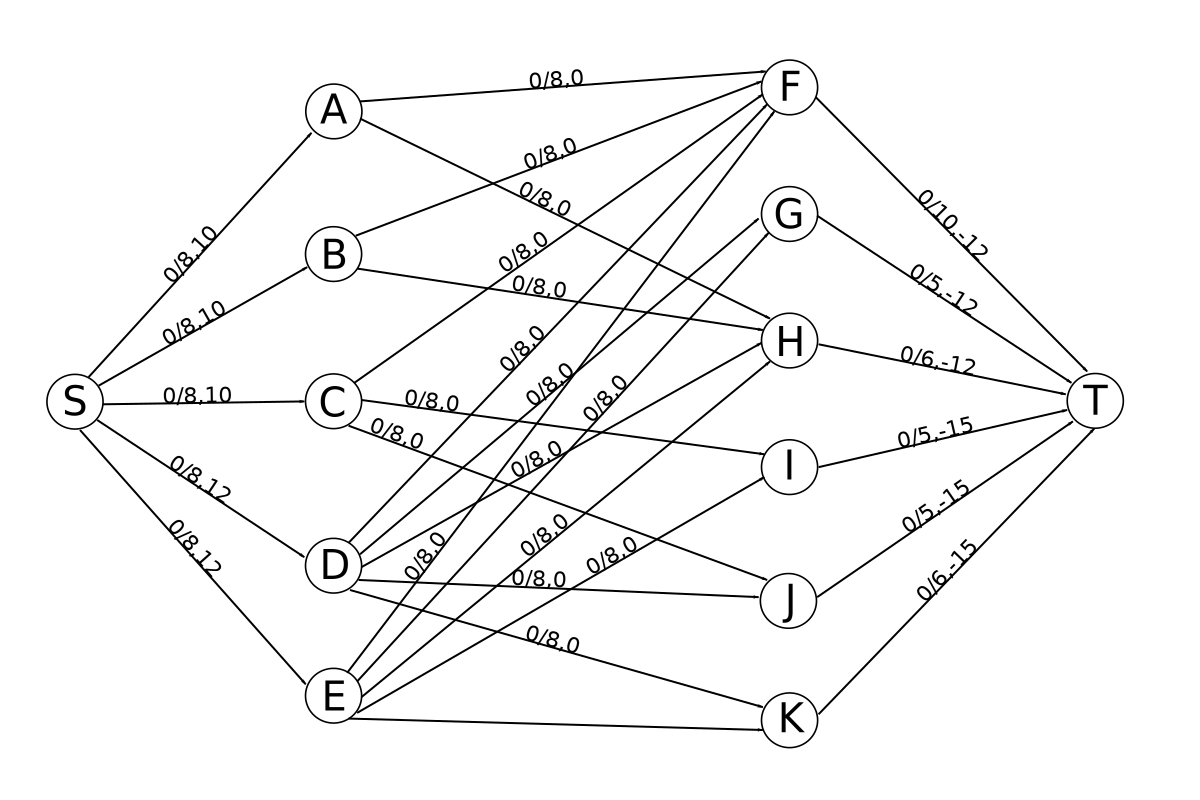
\includegraphics[width=150mm]{cost-graph.png}
\caption{Flussproblem Arbeitsplanung mit Kosten}
\label{overflow}
\end{figure}

Wie in der Abbildung zu erkennen ist, werden den Kanten zusätzlich Kosten (pro Stunde) zugeordnet (die letzte Zahl nach dem Komma), wobei Erträge als negative Kosten auftreten. Für jede Arbeitsstunde entstehen Kosten in Höhe des Stundenlohns des Arbeiters, weswegen diese an den eingehenden Kanten der Arbeiter auftreten. Dabei wird vorausgesetzt, dass die Arbeiter nur für die Stunden bezahlt werden, in welchen sie arbeiten.  \\
Die Kosten an den ausgehenden Kanten der Dienstleistungen stellen die Einnahmen dar, die pro Stunde erzielt werden. Da der Algorithmus später die Kosten minimieren soll, sind sie als negative Werte eingetragen. Somit erhält man durch den Max-Flow Min-Cost Algorithmus einen Wert, der entweder Verlust (wenn positives Ergebnis) oder Gewinn anzeigt (negatives Ergebnis). \\
Alternativ könnte man auch die Kosten an den Kanten, die von der Quelle ausgehen, und den eingehenden Kanten der Senke auf Null setzen und stattdessen auf den Kanten von den Arbeitern zu den Dienstleistungen die jeweilige Differenz von Arbeitslohn und Ertrag der Dienstleistung als Kosten zu setzen.\\

Sollten die Lohnkosten konstant sein, also unabhängig von den geleisteten Arbeitsstunden, könnten sie nicht über den Algorithmus minimiert werden. Stattdessen wären die Kosten aller Kanten von der Quelle und von den Arbeitern gleich Null. Nach Durchlauf des Max-Flow Min-Cost Algorithmus müssten die Lohnkosten ($ 5 * 8 = 40$) als Konstante abgezogen werden um den maximalen Gewinn zu erhalten.\\

Allerdings könnten die negativen Kosten, die in dieser Modellierung verwendet werden, ein Problem darstellen. Sollte der Algorithmus damit nicht arbeiten können, müssten die negativen Kanten entfernt werden. Dies wäre allerdings in diesem Fall nicht möglich, wenn der Algorithmus nur minimale Kosten finden kann: Würde man positive Werte verwenden (also beispielsweise an den Kanten von Arbeitern zu Dienstleistungen je den (positiven) Gewinn pro Stunde: Ertrag der Dienstleistung - Arbeitskosten) müsste der verwendete Algorithmus den maximalen Fluss mit den maximalen "Kosten" (hier Erträgen) finden können.



\end{document}